% Options for packages loaded elsewhere
\PassOptionsToPackage{unicode}{hyperref}
\PassOptionsToPackage{hyphens}{url}
\PassOptionsToPackage{dvipsnames,svgnames,x11names}{xcolor}
%
\documentclass[
  letterpaper,
  DIV=11,
  numbers=noendperiod]{scrartcl}

\usepackage{amsmath,amssymb}
\usepackage{iftex}
\ifPDFTeX
  \usepackage[T1]{fontenc}
  \usepackage[utf8]{inputenc}
  \usepackage{textcomp} % provide euro and other symbols
\else % if luatex or xetex
  \usepackage{unicode-math}
  \defaultfontfeatures{Scale=MatchLowercase}
  \defaultfontfeatures[\rmfamily]{Ligatures=TeX,Scale=1}
\fi
\usepackage{lmodern}
\ifPDFTeX\else  
    % xetex/luatex font selection
\fi
% Use upquote if available, for straight quotes in verbatim environments
\IfFileExists{upquote.sty}{\usepackage{upquote}}{}
\IfFileExists{microtype.sty}{% use microtype if available
  \usepackage[]{microtype}
  \UseMicrotypeSet[protrusion]{basicmath} % disable protrusion for tt fonts
}{}
\makeatletter
\@ifundefined{KOMAClassName}{% if non-KOMA class
  \IfFileExists{parskip.sty}{%
    \usepackage{parskip}
  }{% else
    \setlength{\parindent}{0pt}
    \setlength{\parskip}{6pt plus 2pt minus 1pt}}
}{% if KOMA class
  \KOMAoptions{parskip=half}}
\makeatother
\usepackage{xcolor}
\setlength{\emergencystretch}{3em} % prevent overfull lines
\setcounter{secnumdepth}{-\maxdimen} % remove section numbering
% Make \paragraph and \subparagraph free-standing
\ifx\paragraph\undefined\else
  \let\oldparagraph\paragraph
  \renewcommand{\paragraph}[1]{\oldparagraph{#1}\mbox{}}
\fi
\ifx\subparagraph\undefined\else
  \let\oldsubparagraph\subparagraph
  \renewcommand{\subparagraph}[1]{\oldsubparagraph{#1}\mbox{}}
\fi


\providecommand{\tightlist}{%
  \setlength{\itemsep}{0pt}\setlength{\parskip}{0pt}}\usepackage{longtable,booktabs,array}
\usepackage{calc} % for calculating minipage widths
% Correct order of tables after \paragraph or \subparagraph
\usepackage{etoolbox}
\makeatletter
\patchcmd\longtable{\par}{\if@noskipsec\mbox{}\fi\par}{}{}
\makeatother
% Allow footnotes in longtable head/foot
\IfFileExists{footnotehyper.sty}{\usepackage{footnotehyper}}{\usepackage{footnote}}
\makesavenoteenv{longtable}
\usepackage{graphicx}
\makeatletter
\def\maxwidth{\ifdim\Gin@nat@width>\linewidth\linewidth\else\Gin@nat@width\fi}
\def\maxheight{\ifdim\Gin@nat@height>\textheight\textheight\else\Gin@nat@height\fi}
\makeatother
% Scale images if necessary, so that they will not overflow the page
% margins by default, and it is still possible to overwrite the defaults
% using explicit options in \includegraphics[width, height, ...]{}
\setkeys{Gin}{width=\maxwidth,height=\maxheight,keepaspectratio}
% Set default figure placement to htbp
\makeatletter
\def\fps@figure{htbp}
\makeatother

\KOMAoption{captions}{tableheading}
\makeatletter
\@ifpackageloaded{caption}{}{\usepackage{caption}}
\AtBeginDocument{%
\ifdefined\contentsname
  \renewcommand*\contentsname{Table of contents}
\else
  \newcommand\contentsname{Table of contents}
\fi
\ifdefined\listfigurename
  \renewcommand*\listfigurename{List of Figures}
\else
  \newcommand\listfigurename{List of Figures}
\fi
\ifdefined\listtablename
  \renewcommand*\listtablename{List of Tables}
\else
  \newcommand\listtablename{List of Tables}
\fi
\ifdefined\figurename
  \renewcommand*\figurename{Figure}
\else
  \newcommand\figurename{Figure}
\fi
\ifdefined\tablename
  \renewcommand*\tablename{Table}
\else
  \newcommand\tablename{Table}
\fi
}
\@ifpackageloaded{float}{}{\usepackage{float}}
\floatstyle{ruled}
\@ifundefined{c@chapter}{\newfloat{codelisting}{h}{lop}}{\newfloat{codelisting}{h}{lop}[chapter]}
\floatname{codelisting}{Listing}
\newcommand*\listoflistings{\listof{codelisting}{List of Listings}}
\makeatother
\makeatletter
\makeatother
\makeatletter
\@ifpackageloaded{caption}{}{\usepackage{caption}}
\@ifpackageloaded{subcaption}{}{\usepackage{subcaption}}
\makeatother
\ifLuaTeX
  \usepackage{selnolig}  % disable illegal ligatures
\fi
\usepackage{bookmark}

\IfFileExists{xurl.sty}{\usepackage{xurl}}{} % add URL line breaks if available
\urlstyle{same} % disable monospaced font for URLs
\hypersetup{
  pdftitle={Análise de Mercado para Cibersegurança e DevOps},
  pdfauthor={Arthur Morelo},
  colorlinks=true,
  linkcolor={blue},
  filecolor={Maroon},
  citecolor={Blue},
  urlcolor={Blue},
  pdfcreator={LaTeX via pandoc}}

\title{Análise de Mercado para Cibersegurança e DevOps}
\author{Arthur Morelo}
\date{}

\begin{document}
\maketitle

\subsection{Introdução}\label{introduuxe7uxe3o}

O mercado de tecnologia tem passado por uma transformação significativa
nos últimos anos, migrando de uma demanda massiva por desenvolvimento de
software genérico para a especialização em nichos de alta criticidade.
Dentre estes, Cibersegurança e DevOps destacam-se como pilares
fundamentais para a garantia de resiliência, escalabilidade e proteção
de dados nas operações corporativas modernas. A crescente complexidade
das ameaças digitais e a necessidade de entregas contínuas e
automatizadas tornam esses profissionais peças-chave no ecossistema
tecnológico atual.

Para compreender a fundo essa dinâmica de mercado, foi realizada uma
ampla extração e análise de dados provenientes de fontes diversificadas,
como LinkedIn, CIEE e Jobbol. Essa abordagem multiplataforma permitiu
capturar desde oportunidades de estágio até posições sêniores de
engenharia e arquitetura, oferecendo uma visão panorâmica e realista
sobre o volume de vagas, a remuneração média e os principais desafios
enfrentados pelos profissionais destas áreas de infraestrutura.

\subsection{Requisições do Mercado}\label{requisiuxe7uxf5es-do-mercado}

A partir da aplicação de técnicas de Processamento de Linguagem Natural
(NLP) sobre as descrições das vagas, foi possível extrair a frequência
das principais habilidades exigidas pelo mercado. A análise do gráfico
de requisições revela que ferramentas de orquestração de contêineres e
fundamentos de sistemas operacionais dominam os requisitos das vagas. O
domínio de tecnologias como Kubernetes, Docker, Linux e provedores de
nuvem pública (AWS) tornou-se mandatório, evidenciando uma transição de
profissionais puramente focados em código para especialistas capazes de
projetar, automatizar e proteger infraestruturas complexas e
distribuídas.

\subsection{Motores de Recuperação de Informação
(RI)}\label{motores-de-recuperauxe7uxe3o-de-informauxe7uxe3o-ri}

A eficiência na localização de oportunidades adequadas depende
diretamente do motor de busca utilizado. Na análise, avaliamos três
abordagens distintas de Recuperação de Informação:

\begin{itemize}
\tightlist
\item
  \textbf{Score Booleano:} É o modelo mais elementar de RI, baseado na
  teoria de conjuntos. Ele calcula a relevância através da presença ou
  ausência exata dos termos da consulta (\emph{query}) no documento. Se
  a palavra exata não estiver no texto, o documento é sumariamente
  ignorado, sem meio-termo ou cálculo de similaridade semântica.
\item
  \textbf{Score BM25 (Best Matching 25):} Representa o estado da arte
  dos modelos probabilísticos baseados em frequência de termos (TF-IDF).
  Ele não apenas verifica a presença da palavra-chave, mas também
  pondera a frequência com que o termo aparece no documento em relação à
  sua raridade em toda a coleção de vagas, penalizando documentos
  excessivamente longos para manter a precisão do ranqueamento.
\item
  \textbf{Score de Embeddings:} Utiliza redes neurais profundas
  (arquitetura Transformer) para converter textos e consultas em vetores
  matemáticos densos em um espaço n-dimensional. A relevância é
  calculada pela similaridade do cosseno entre os vetores. Este modelo
  não busca correspondência exata de palavras, mas sim a similaridade
  semântica, conseguindo relacionar termos sinônimos ou conceitos
  próximos dentro de um mesmo contexto técnico.
\end{itemize}

\subsection{Visualização de Dados}\label{visualizauxe7uxe3o-de-dados}

\begin{figure}[H]

{\centering 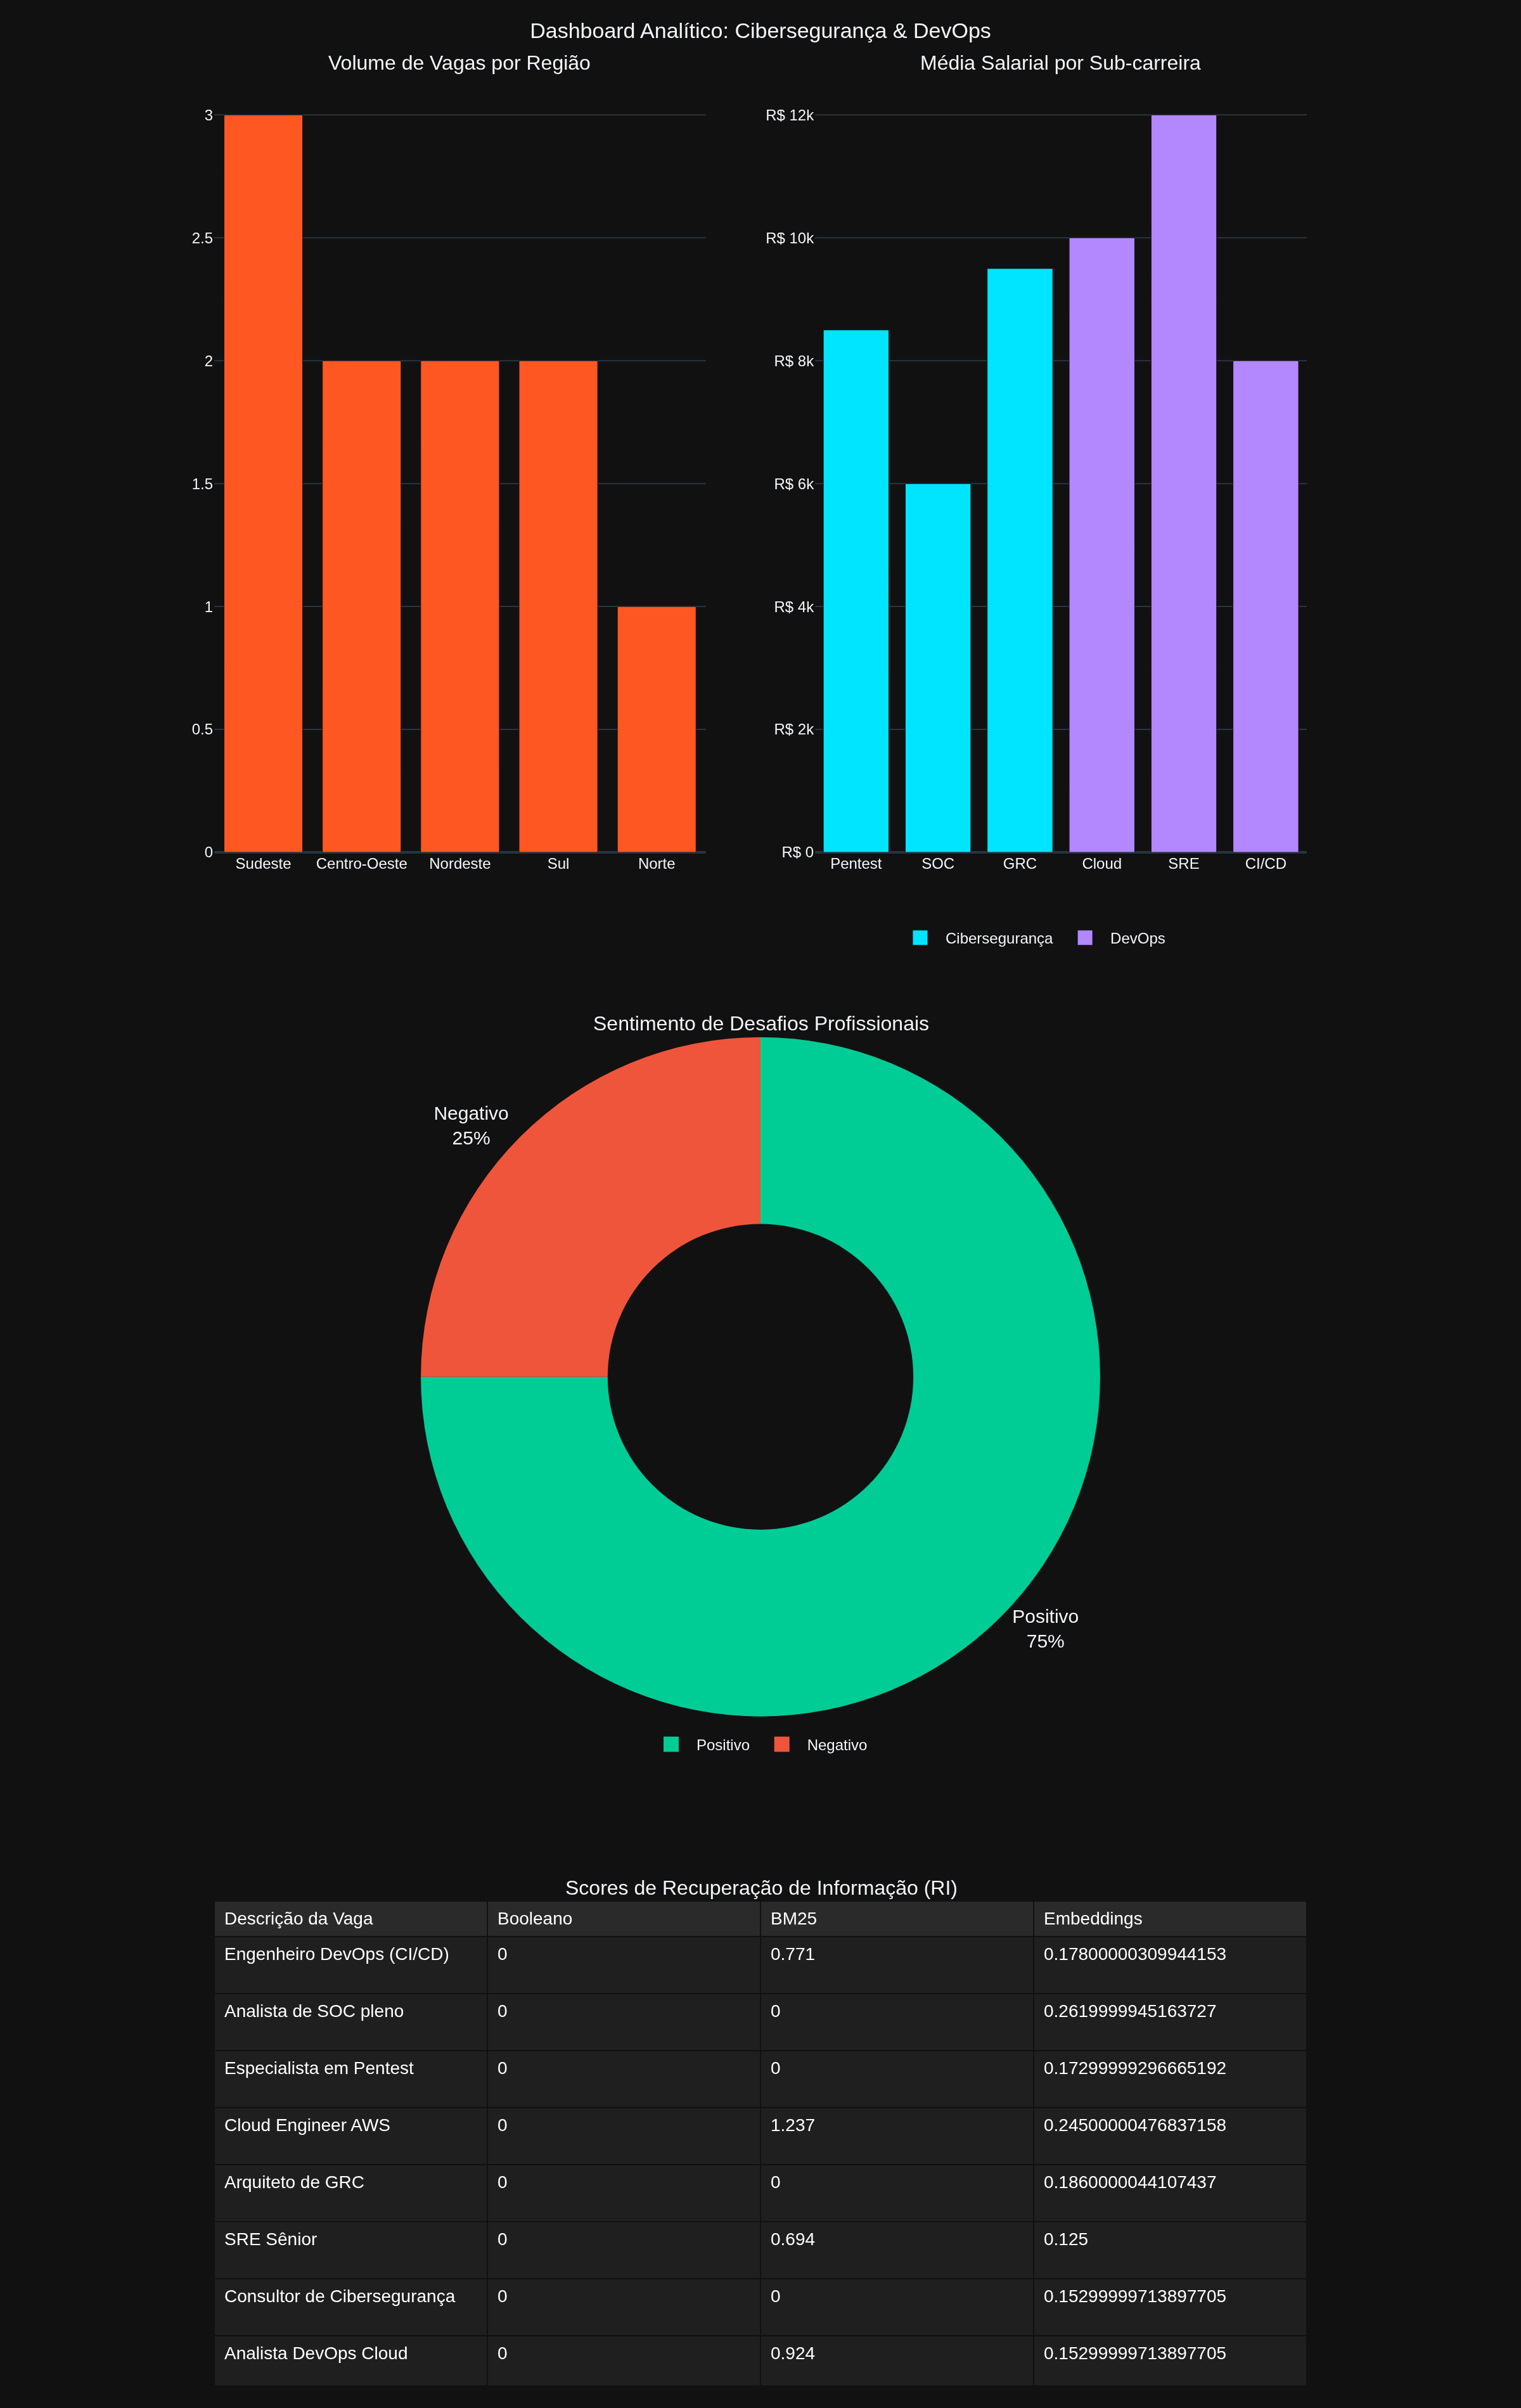
\includegraphics[width=1\textwidth,height=\textheight]{../output/dashboard_cybersec.png}

}

\caption{Dashboard Analítico de Cibersegurança e DevOps}

\end{figure}%

\subsection{Conclusão: Recuperação de Informação e
NLP}\label{conclusuxe3o-recuperauxe7uxe3o-de-informauxe7uxe3o-e-nlp}

A análise das descrições de vagas demonstrou de forma clara as
limitações das abordagens tradicionais de busca em comparação com as
tecnologias modernas de Processamento de Linguagem Natural (NLP). O
modelo Booleano de Recuperação de Informação (RI), por basear-se na
correspondência exata de palavras-chave, frequentemente falha ao lidar
com a riqueza de vocabulário da área de infraestrutura. Se uma vaga
requisita conhecimentos em ``Containers'', uma busca Booleana estrita
pela palavra ``Docker'' não a recuperaria.

Por outro lado, o modelo baseado em Embeddings semânticos apresentou
resultados vastamente superiores na identificação de oportunidades. Ao
projetar os textos em um espaço vetorial de alta dimensionalidade, o
modelo de Embeddings é capaz de compreender o contexto e a intenção
subjacente nas descrições. Dessa forma, ele identifica com precisão a
correlação semântica entre termos técnicos --- compreendendo, por
exemplo, que ``Docker'' e ``Containers'', ou ``AWS'' e ``Cloud'',
referem-se a conceitos intimamente ligados. Essa capacidade de abstração
e entendimento de contexto torna a extração e recomendação de vagas de
DevOps e Cibersegurança muito mais inteligentes, assertivas e aderentes
à realidade do mercado.



\end{document}
